\section{Equilibrio Líquido-Vapor}\label{sec:heterogeneous}

	La clase `Heterogeneous' se encarga de los cálculos de equilibrio entre las fases líquido y vapor. La clase contiene dos instancias de la clase `Homogeneous' que representan a la clase líquida y a la clase vapor. La clase implementa los algoritmos numéricos para igualar los cálculos de la fugacidad entre las fases.

	Los cálculos de equilibrio que se implementan en este trabajo son:

	\begin{itemize}

		\item Substancias
			\begin{itemize}
				\item Temperatura de saturación.
				\item Presión de saturación.
			\end{itemize}

		\item Mezclas
	\begin{itemize}
		\item Presión de burbuja, sección \ref{subsec:bubblepressure}.
		\item Presión de rocío, sección \ref{subsec:dewpressure}.
		\item Temperatura de burbuja, sección \ref{subsec:bubbletemperature}.
		\item Temperatura de rocío, sección \ref{subsec:dewtemperature}.
		\item Flash temperatura-presión \ref{subsec:flash}.
	\end{itemize}

	\end{itemize}

	Los algoritmos son muy similares, las principales diferencias consisten en la función objetivo.

	La clase `HeterogeneousSubstance' realiza los cálculos de equilibrio para las substancias y la clase `HeterogeneousSubstance' realiza los cálculos de equilibrio para las mezclas, en la figura \ref{fig:heterogeneous} ser muestra la estructura.

\begin{figure}[!h]
  \centering
    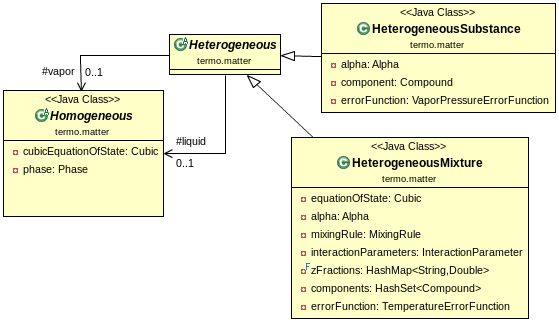
\includegraphics[scale=0.7]{heterogeneous.png}
    \caption{Estructura de la librería para el cálculo de equilibrio Líquido-Vapor.}
    \label{fig:heterogeneous}
\end{figure}

	Los cálculos de la presente sección se realizan de forma muy similar, primero indicando la variable conocida con el método `set', después invocando el método que realiza el algoritmo para conocer la incognita, el método puede recibir o no un estimado inicial y finalmente obtener el resultado de la variable con el método `get'.

	Cada sección muestra el uso de la librería con fragmentos de código que realizan el cálculo con y sin el estimado inicial. También se indica que método se usa para estimar la varible incognita en caso de no proporcionar un estimado inicial.

		
